% ---------------------------------------------------------------------
\subsection{Mockup delle Interfacce Utente}
\label{sec:mockup}
% ---------------------------------------------------------------------

Questa sezione presenta i mockup delle interfacce principali del sistema \productname. I mockup mostrano il layout e il flusso di interazione delle schermate.

% ---------------------------------------------------------------------
\subsubsection{Mockup Creazione Issue}
\label{subsec:mockup-creazione-issue}
% ---------------------------------------------------------------------

La Figura sottostante mostra il flusso completo di creazione di una nuova issue, includendo il form principale e i messaggi di feedback (successo ed errori).

\begin{figure}[H]
\centering
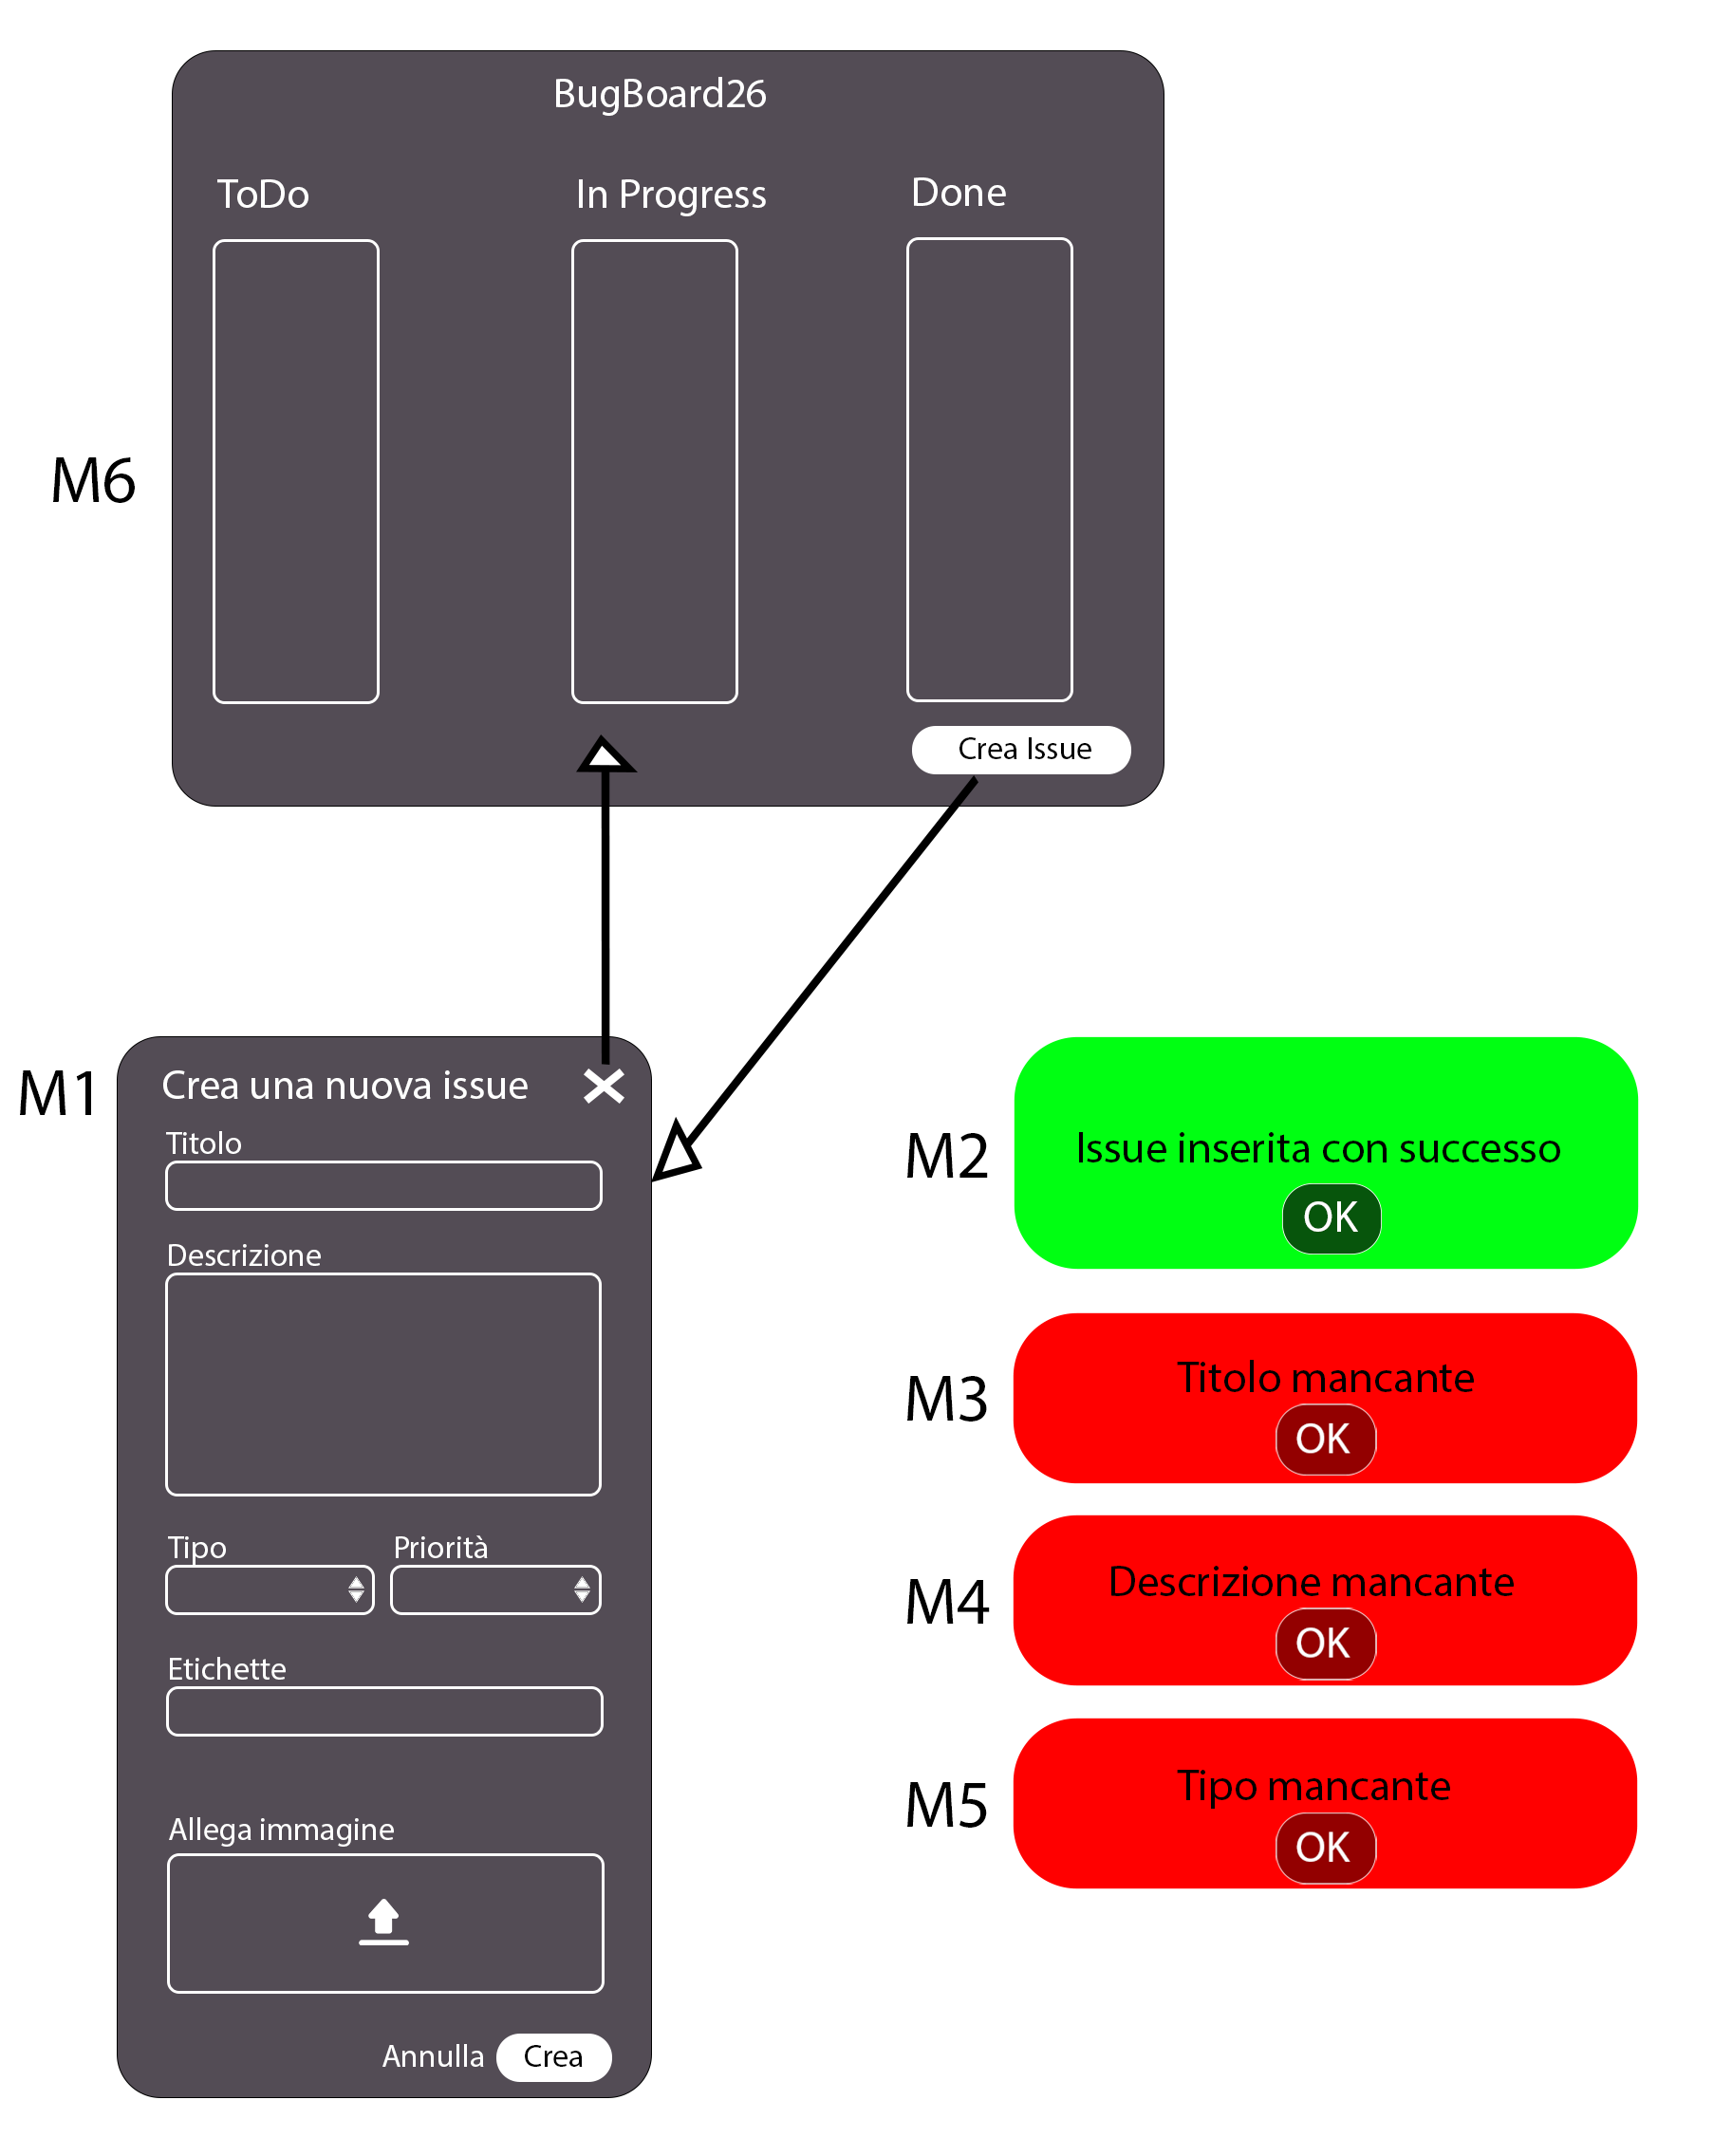
\includegraphics[width=0.7\textwidth]{MOCK.png}
\caption{Mockup flusso creazione issue. La figura mostra:
\textbf{M1} - Form creazione con campi Titolo, Descrizione, Tipo, Priorità, Etichette e Upload immagini;
\textbf{M2} - Messaggio successo "Issue inserita con successo";
\textbf{M3} - Errore "Titolo mancante";
\textbf{M4} - Errore "Descrizione mancante";
\textbf{M5} - Errore "Tipo mancante";
\textbf{M6} - Vista board Kanban con colonne ToDo, In Progress, Done.}
\label{fig:mock-issue}
\end{figure}

% ---------------------------------------------------------------------
\subsubsection{Descrizione Schermate}
\label{subsec:descrizione-schermate}
% ---------------------------------------------------------------------

\paragraph{M1 - Form Creazione Issue}

Form principale per creare nuove issue nel progetto corrente.

\paragraph{Elementi}
\begin{itemize}[leftmargin=1.1em]
\item Header "Crea una nuova issue" con pulsante chiusura (X)
\item Campo Titolo (obbligatorio, input testo singola riga)
\item Campo Descrizione (obbligatorio, textarea multiriga)
\item Dropdown Tipo (obbligatorio: Bug, Feature, Question, Documentation)
\item Dropdown Priorità (opzionale: Nessuna, Bassa, Media, Alta, Critica)
\item Campo Etichette (opzionale)
\item Area upload immagini
\item Pulsanti "Annulla" e "Crea" in basso
\end{itemize}

\paragraph{M2 - Conferma Successo}

Toast notification che appare dopo la creazione con successo della issue.

\subparagraph{Contenuto}
\begin{itemize}[leftmargin=1.1em]
\item Testo "Issue inserita con successo"
\item Pulsante "OK"
\item Scompare automaticamente dopo 3 secondi o al click su OK
\end{itemize}

\subsubsection{M3, M4, M5 - Messaggi Errore}

Alert che appaiono quando mancano campi obbligatori.

\subparagraph{Contenuto}
\begin{itemize}[leftmargin=1.1em]
\item M3: "Titolo mancante"
\item M4: "Descrizione mancante"
\item M5: "Tipo mancante"
\item Pulsante "OK" per chiudere
\item Il campo mancante viene evidenziato in rosso nel form
\end{itemize}

\subsubsection{M6 - Board Kanban}

Vista alternativa delle issue organizzate in colonne per stato.

\subparagraph{Elementi}
\begin{itemize}[leftmargin=1.1em]
\item Header "BugBoard26"
\item Almeno tre colonne: "ToDo", "In Progress", "Done"
\item Pulsante "Crea Issue" in basso a destra
\end{itemize}

\subparagraph{Note}
La board Kanban è una vista alternativa alla lista tabellare, in cui sono presenti colonne corrispettive agli stati con all'interno le varie issue. Le issue possono essere spostate tra colonne con drag\&drop per cambiare lo stato in modo efficiente.

% ---------------------------------------------------------------------
\subsubsection{Principi di Design}
\label{subsec:principi-design}
% ---------------------------------------------------------------------

I mockup seguono questi principi:

\begin{itemize}[leftmargin=1.1em]
\item \textbf{Semplicità}: layout pulito con elementi essenziali
\item \textbf{Feedback immediato}: messaggi di successo/errore chiari
\item \textbf{Validazione}: campi obbligatori evidenziati quando mancanti
\end{itemize}
